% CHAPTER 6: SYSTEM INTEGRATION AND DEPLOYMENT
% ======================================================================
{\fontsize{18}{22}\selectfont\textbf{6 System Integration and Deployment}}\par

\vspace{3mm}

\subhead{6.1 User Center and RBAC}

The user center (user service, port 8081) integrates identity management, access control, department-level data isolation, as well as cross-cutting notification and document services. Table 26 shows the dual-mode login and JWT session management flow.

\vspace{3mm}

\needspace{6\baselineskip}
\begin{center}
\textbf{Table 26: Pseudocode --- Dual-Mode Login and JWT Session Management}
\end{center}

\begin{lstlisting}
// === Dual-Mode Login ===
ENDPOINT POST /user/login  ->  {username, password, code?}
FUNCTION login(username, password, code): AuthResult
    IF code IS PROVIDED THEN
        // Mode 1 - Email verification code login
        storedCode = redis.get("email:code:" + username)
        IF storedCode IS NULL OR storedCode <> code THEN
            THROW InvalidCodeException()
        END IF
        redis.delete("email:code:" + username)  // single-use
    ELSE
        // Mode 2 - Password login with BCrypt verification
        user = userMapper.selectByUsername(username)
        IF user IS NULL OR NOT BCrypt.matches(password, user.password) THEN
            THROW BadCredentialsException()
        END IF
    END IF
    roles = roleMapper.selectByUserId(user.id)
    perms = permissionMapper.selectByRoles(roles)
    token = jwtService.generate({
        sub:      username,
        roles:    roles,
        perms:    perms,
        deptId:   user.deptId,
        clearLv:  user.clearanceLevel,
        exp:      now() + 24h
    })
    redis.set("session:active:" + username, token, {ttl: 30min})
    RETURN {token, username, roles, permissions, realName}
END FUNCTION

// === Gateway JWT Validation (JwtAuthGlobalFilter, order = -100) ===
FUNCTION filter(exchange, chain):
    IF requestPath IN whitelist THEN  // /login, /register, /send-code
        RETURN chain.filter(exchange)
    END IF
    token = extractBearerToken(request)
    claims = jwtService.validateAndParse(token)
    session = redis.get("session:active:" + claims.sub)
    IF session IS NULL THEN THROW SessionExpiredException()
    // Inject downstream headers
    request.mutateHeader("X-User-Name",        claims.sub)
    request.mutateHeader("X-User-Roles",       join(claims.roles))
    request.mutateHeader("X-User-Permissions", join(claims.perms))
    // Sliding-window renewal (exclude polling endpoints)
    IF NOT requestPath.contains("/notification/unread-count") THEN
        redis.expire("session:active:" + claims.sub, 30min)
    END IF
    RETURN chain.filter(exchange)
END FUNCTION
\end{lstlisting}


Access Control. Three roles (ROLE\_ADMIN, ROLE\_DEPT\_ADMIN, ROLE\_USER) and six granular permissions are used to control access to all protected endpoints. The six departments (Credit Department, Compliance Department, Asset Management Department, Retail Banking Department, Investment Banking Department, and Risk Control Department) provide organizational data scoping. A custom JwtAuthenticationFilter extracts permissions from JWT claims and registers them in Spring Security's SecurityContextHolder. The @PreAuthorize annotation on each controller method can be declared with hasAuthority checks, while the abstraction level's department admin controllers additionally verify that the requested resource's dept\_id matches the accessing user's dept\_id, enabling cross-cutting department-level data isolation.

\subhead{6.2 Task Center and Orchestration}

The task center sends requests to the agent, tracks the execution progress and returns the results. The orchestration function is distributed between the gateway (static routing) and each agent service (autonomous execution).When a user submits a task through the Copilot or an agent page, the task is persisted, queued for asynchronous execution, and progress is pushed through WebSocket. A retry queue with exponential backoff provides fault tolerance, while a fixed-size thread pool (configurable, default 10 threads) limits concurrency.

\subhead{6.3 WebSocket Real-Time Communication}

Long-running AI tasks need progress streaming beyond HTTP request-response. The platform uses WebSocket connections to push task progress from backend to frontend.

Figure 10 shows the WebSocket task progress architecture, illustrating how long-running AI task progress is pushed from the backend TaskProgressWebSocketHandler to the frontend in real time via WebSocket connections proxied through the Spring Cloud Gateway.

Table 27 shows the WebSocket-based task progress streaming mechanism with step-by-step JSON push and frontend rendering.

\vspace{3mm}

\needspace{6\baselineskip}
\begin{center}
\textbf{Table 27: Pseudocode --- TaskProgressWebSocketHandler Real-Time Progress Streaming}
\end{center}

\begin{lstlisting}
// === Backend: TaskProgressWebSocketHandler ===
// Registered at /tool/ws via WebSocketConfig

CLASS TaskProgressWebSocketHandler EXTENDS TextWebSocketHandler:
    sessions = ConcurrentHashMap<String, WebSocketSession>()

    FUNCTION afterConnectionEstablished(session):
        taskId = extractQueryParam(session.uri, "taskId")
        sessions.put(taskId, session)
        executor.submit(() -> simulateProgress(taskId, session))
    END FUNCTION

    FUNCTION simulateProgress(taskId, session):
        FOR step IN [1..5]:
            sleep(500ms)
            progress = {taskId: taskId, step: step, total: 5,
                        message: "Processing step " + step + "/5"}
            session.sendMessage(new TextMessage(toJSON(progress)))
        END FOR
        sessions.remove(taskId)
    END FUNCTION
END CLASS

// === Frontend: WebSocket Client ===
// Singleton at utils/websocket.ts
FUNCTION connectWebSocket(taskId):
    ws = new WebSocket(BASE_WS_URL + "/tool/ws?taskId=" + taskId)
    ws.onmessage = (event) -> {
        progress = JSON.parse(event.data)
        agentThinking.updateSteps(progress)
        IF progress.step = progress.total THEN
            fetchTaskResult(taskId)  // via AgentThinking.vue
        END IF
    }
END FUNCTION

// Gateway proxy: /ws/** -> tool-agent:8083/tool/ws
// JWT passed as query parameter; upgrade requests whitelisted
\end{lstlisting}


\subhead{6.4 Containerized Deployment}

Figure 10 shows the Docker Compose service topology, illustrating how each service (Gateway, four backend microservices, frontend, MySQL, Redis, and optionally Milvus with etcd and MinIO) runs in an independent container on an internal Docker network, with only the Gateway port exposed externally.

\begin{figure}[H]
\centering
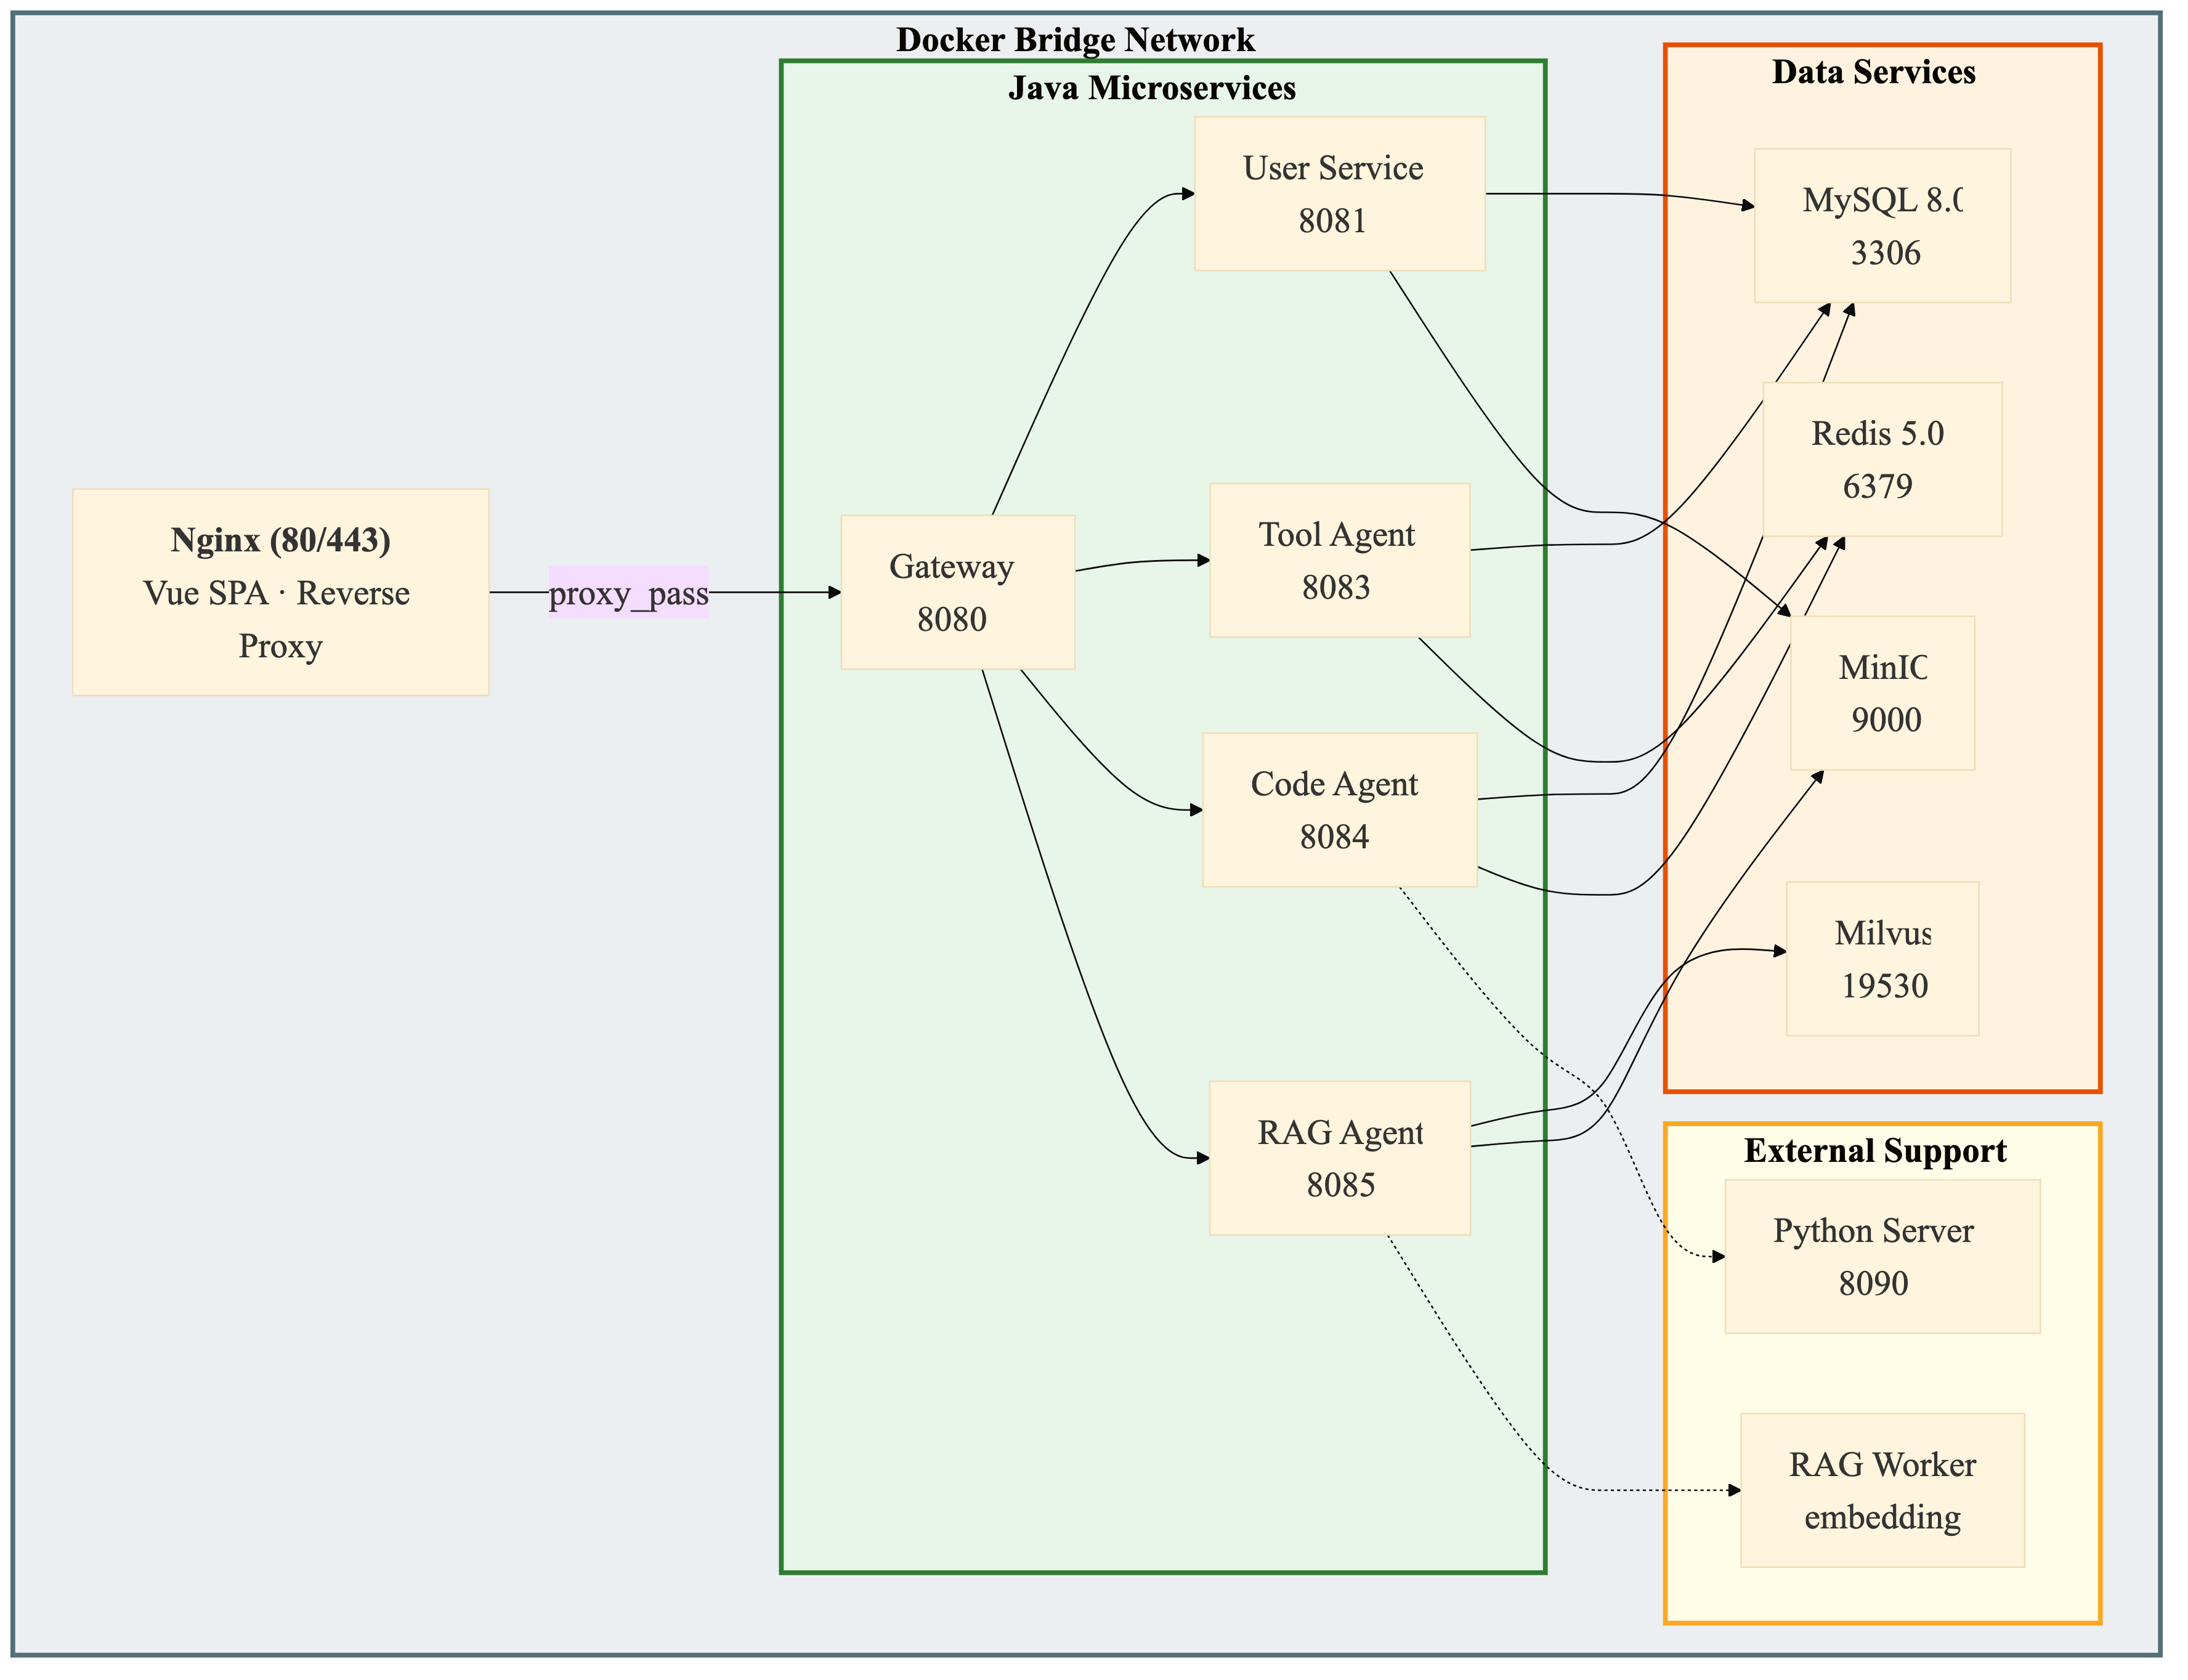
\includegraphics[width=0.92\textwidth]{figures/fig10_docker_topology.png}
\caption{Docker Compose Service Topology}
\end{figure}

The platform is deployed through Docker Compose. Each service (Gateway, four backend services, frontend, MySQL, Redis, and optionally Milvus with etcd and MinIO) runs in an independent container on an internal bridge network. Only the Gateway (port 8080) is exposed. The frontend Nginx (port 80) serves static Vue 3 SPA files and proxies API and WebSocket requests to the Gateway. MySQL initialization is handled via a mounted SQL dump file. The Python inference server for the Code Agent runs in a separate container with FastAPI.

\newpage

% ======================================================================
